% (c) 2002 Matthew Boedicker <mboedick@mboedick.org> (original author) http://mboedick.org
% (c) 2003-2007 David J. Grant <davidgrant-at-gmail.com> http://www.davidgrant.ca
% (c) 2008 Nathaniel Johnston <nathaniel@nathanieljohnston.com> http://www.nathanieljohnston.com
% (c) 2011 Scott Clark <sc932@cornell.edu> http://cam.cornell.edu/~sc932
% (c) 2012 Arne Hassel <arne.hassel@gmail.com> http://megoth.wordpress.com/
%
%This work is licensed under the Creative Commons Attribution-Noncommercial-Share Alike 2.5 License. To view a copy of this license, visit http://creativecommons.org/licenses/by-nc-sa/2.5/ or send a letter to Creative Commons, 543 Howard Street, 5th Floor, San Francisco, California, 94105, USA.

\documentclass[letterpaper,11pt,norsk]{article}
\newlength{\outerbordwidth}
\pagestyle{empty}
\raggedbottom
\raggedright
\usepackage{array}
\usepackage{babel}
\usepackage{colortbl}
\usepackage{color}
\usepackage{float}
\usepackage[T1]{fontenc}
\usepackage{framed}
\usepackage{graphicx}
\usepackage{ifthen}
\usepackage[utf8]{inputenc}
\usepackage{tocloft}
\usepackage{url}
\usepackage[svgnames]{xcolor}
\usepackage{wrapfig}

%-----------------------------------------------------------

%Edit these values as you see fit

\setlength{\outerbordwidth}{3pt}  % Width of border outside of title bars
\definecolor{shadecolor}{gray}{0.75}  % Outer background color of title bars (0 = black, 1 = white)
\definecolor{shadecolorB}{gray}{0.93}  % Inner background color of title bars

%-----------------------------------------------------------

%Margin setup

\newlength{\cellwidth}
\newlength{\colmainwidth}
\newlength{\tablewidth}

\setlength{\cellwidth}{0.2in}
\setlength{\colmainwidth}{3.4in}
\setlength{\evensidemargin}{-0.25in}
\setlength{\headheight}{-0.25in}
\setlength{\headsep}{0in}
\setlength{\oddsidemargin}{-0.25in}
\setlength{\paperheight}{11in}
\setlength{\paperwidth}{8.5in}
\setlength{\tablewidth}{7in}
\setlength{\tabcolsep}{0in}
\setlength{\textheight}{9.75in}
\setlength{\textwidth}{7in}
\setlength{\topmargin}{-0.3in}
\setlength{\topskip}{0in}
\setlength{\voffset}{0.1in}

%-----------------------------------------------------------

%Custom commands

\newcommand{\resitem}[1]{\item #1 \vspace{-2pt}}

\newcommand{\resheading}[1]{\vspace{8pt}
  \parbox{\textwidth}{\setlength{\FrameSep}{\outerbordwidth}
    \begin{shaded}
\setlength{\fboxsep}{0pt}\framebox[\textwidth][l]{\setlength{\fboxsep}{4pt}\fcolorbox{shadecolorB}{shadecolorB}{\textbf{\sffamily{\mbox{~}\makebox[6.762in][l]{\large #1} \vphantom{p\^{E}}}}}}
    \end{shaded}
  }\vspace{-5pt}
}

\newcommand{\ressubheading}[4]{
\begin{tabular*}{6.5in}{l@{\cftdotfill{\cftsecdotsep}\extracolsep{\fill}}r}
		\textbf{#1} & #2 \\
		\textit{#3} & \textit{#4} \\
\end{tabular*}\vspace{-6pt}}

\newcommand{\forloop}[6][1]%
{%
\setcounter{#2}{#3}%
\ifthenelse{#4}%
	{%
	#6%
	\ifthenelse{#5}{\arabic{#2}}{\hspace{3mm}}
	\addtocounter{#2}{#1}%
	\forloop[#1]{#2}{\value{#2}}{#4}{#5}{#6}%
	}%
% Else
	{%
	}%
}%

\newcounter{ct}
\newcounter{kl}
\newcounter{klm}
\newcounter{wl}
\newcounter{wlm}
\newcommand{\skill}[3]{
	\setcounter{ct}{-1}
	\setcounter{kl}{#2}
	\setcounter{klm}{#2}
	\setcounter{wl}{#3}
	\setcounter{wlm}{#3}
	
	\addtocounter{klm}{1}
	\addtocounter{wlm}{1}
	
	#1
	\forloop{ct}{1}{\value{ct} < \value{klm}}{\value{ct} = \value{kl}}%
	{%
	& \cellcolor[gray]{0.5}
	}
	\forloop{ct}{\value{klm}}{\value{ct} < \value{wlm}}{\value{ct} = \value{wl}}%
	{%
	& \cellcolor[gray]{0.9}
	}
	\forloop{ct}{\value{wlm}}{\value{ct} < 11}{\value{ct} = 11}%
	{%
	& \cellcolor[gray]{1}
	}
	\\
}

\newcommand{\skilltable}[2]{
	\vspace{2.5mm}
	\begin{tabular}{p{1.5in} l*{10}{c}}
		\textbf{\Large #1} & 1 & 2 & 3 & 4 & 5 & 6 & 7 & 8 & 9 & 10 \\
		\hline
		#2
	\end{tabular}
}

%-----------------------------------------------------------

\title{Curriculum Vitae}

\begin{document}

\begin{minipage}{\textwidth}
\begin{wrapfigure}{r}{0pt}
	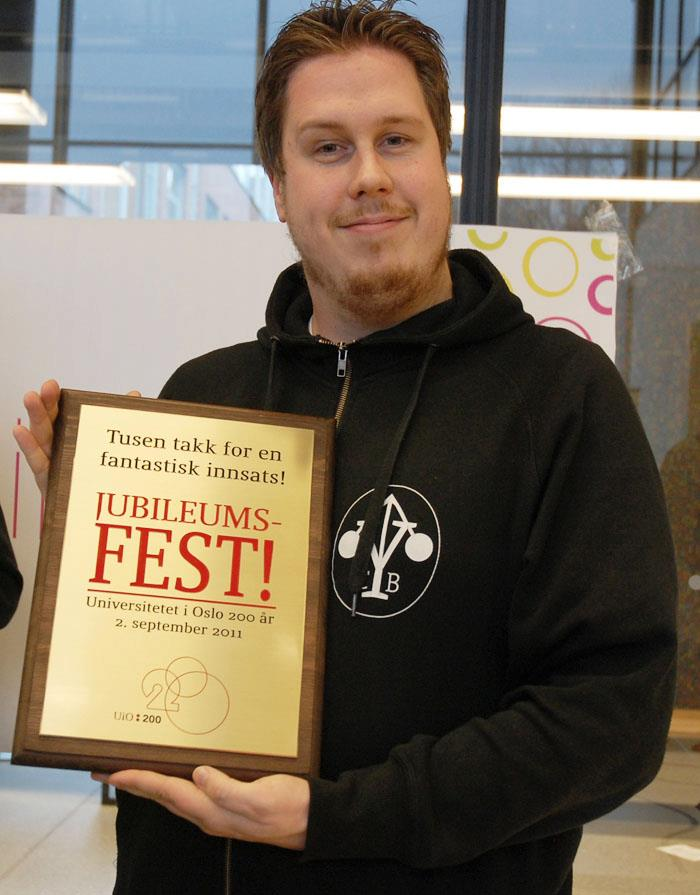
\includegraphics[height=45mm]{uio200.jpg}
\end{wrapfigure}

\textbf{\Large Competanse chart for Arne Hassel}

\vspace{5mm}

\begin{minipage}{5in}
The competence chart provide an overview of my skills both professionally, personally and socially. It is an extension of my resume and provide a better overview in the different areas of expertise. The diagrams are self-critical and personal, and uses a scale from 0 to 10 in order to emphasize how good the skills I have in the different areas are. 0, no hatching, means no qualifications and 10, fully shaded, means maximum expertise in a field. Areas in which I'm interested in and want to improve myself in are shaded in a lighter color to the level I want to reach.
\end{minipage}

\end{minipage}

\resheading{Computer science}

\begin{tabular*}{\tablewidth}{p{\colmainwidth}@{\extracolsep{\fill}}p{\colmainwidth}}
\skilltable{Theory}{%
	\skill{Algorithms}{4}{7}
	\skill{Databases}{7}{9}
	\skill{Computer architecture}{3}{5}
	\skill{Datastructures}{6}{7}
	\skill{Design patterns}{7}{9}
	\skill{Logic}{4}{8}
	\skill{Mathematics}{5}{8}
	\skill{Modeling}{7}{8}
	\skill{Qualitative research}{6}{7}
	\skill{Semantic technologies}{7}{9}
	\skill{Statistics}{3}{6}
	\skill{System development}{7}{10}
}%
&
\skilltable{Programming}{%
	\skill{Assembly}{2}{2}
	\skill{C}{4}{6}
	\skill{C\#}{5}{8}
	\skill{Documentation}{5}{9}
	\skill{Java}{5}{6}
	\skill{JavaScript}{5}{10}
	\skill{PHP}{4}{6}
	\skill{Python}{4}{9}
	\skill{Regex}{3}{9}
	\skill{SPARQL}{4}{7}
	\skill{SQL}{6}{7}
	\skill{Testing (TDD)}{5}{9}
	\skill{XSLT}{5}{5}
}%
\\
\skilltable{Stylesheet}{%
	\skill{CSS}{8}{10}
	\skill{LESS}{6}{8}
	\skill{Sass}{5}{8}
}% 
&
\skilltable{Markup}{%
	\skill{HTML}{8}{10}
	\skill{Turtle}{8}{9}
	\skill{XML}{5}{5}
}% 
\\
\skilltable{Design}{%
	\skill{Design for mobile}{5}{9}
	\skill{Graphic design}{3}{5}
	\skill{Informationdesign}{6}{9}
	\skill{Interactiondesign}{5}{8}
	\skill{Responsive design}{7}{10}
}% 
&
\skilltable{Framework}{%
	\skill{Compass}{6}{9}
	\skill{Django}{3}{8}
	\skill{jQuery}{7}{10}
	\skill{.NET MVC}{5}{8}
	\skill{Umbraco}{5}{5}
	\skill{Wordpress}{4}{6}
}% 
\\
\skilltable{OS}{%
	\skill{OSX}{6}{7}
	\skill{Ubuntu Linux}{4}{9}
	\skill{Windows 7}{8}{8}
	\skill{Windows Vista}{7}{7}
	\skill{Windows XP}{8}{8}
}%
&
\skilltable{Program suites}{%
	\skill{MS Office}{8}{8}
	\skill{Open Office}{6}{7}
	\skill{Photoshop CS4}{4}{6}
	\skill{Visual Studio}{7}{9}
}% 
\end{tabular*}

\resheading{Personal}

\begin{tabular*}{\tablewidth}{p{\colmainwidth}@{\extracolsep{\fill}}p{\colmainwidth}}
\skilltable{Attributes}{%
	\skill{Analytical}{6}{8}
	\skill{Balanced}{7}{7}
	\skill{Concientious}{7}{7}
	\skill{Creative}{6}{8}
	\skill{Curious}{8}{8}
	\skill{Efficient}{7}{8}
	\skill{Independent}{8}{8}
	\skill{Loyal}{9}{9}
	\skill{Positive attitude}{7}{7}
	\skill{Reasonable}{7}{7}
	\skill{Responsible}{7}{7}
	\skill{Structured}{7}{8}
}%
&
\skilltable{Ability to:}{%
	\skill{Acquire knowledge}{7}{10}
	\skill{Cooperate}{7}{8}
	\skill{Dealing with adversity}{7}{8}
	\skill{Give criticism}{6}{8}
	\skill{Give credit}{5}{8}
	\skill{Listen}{5}{8}
	\skill{Motivate others}{7}{7}
	\skill{Say no}{8}{8}
}%
\\
\skilltable{Sosial}{%
	\skill{Accommodating}{7}{7}
	\skill{Companionable}{6}{6}
	\skill{Inclusive}{8}{8}
	\skill{Outgoing}{6}{6}
	\skill{Service minded}{7}{7}
}%
\end{tabular*}

\resheading{Annet}

\begin{tabular*}{\tablewidth}{p{\colmainwidth}@{\extracolsep{\fill}}p{\colmainwidth}}
\skilltable{Administration}{%
	\skill{Management}{5}{9}
	\skill{Organizational analysis}{3}{7}
	\skill{Risk analysis}{3}{7}
	\skill{SWOT-analysis}{3}{5}
}%
&
\skilltable{Economics}{%
	\skill{Accounting}{7}{7}
	\skill{Budgets}{6}{7}
	\skill{Journal keeping}{7}{7}
	\skill{Macro economics}{5}{5}
}%
\\
\skilltable{Languages}{%
	\skill{English}{8}{10}
	\skill{Norwegian}{9}{10}
}%
\\
\end{tabular*}

\end{document}
